\documentclass[aspectratio=169,11pt]{beamer}

\usepackage[utf8]{inputenc}
\usepackage[T1]{fontenc}
\usepackage{amsmath,amssymb}
\usepackage{graphicx}
\usepackage{booktabs}
\usepackage{ctex}   % comment out if ctex unavailable; English alt provided below in [..]

\usetheme{Madrid}
\usecolortheme{seahorse}
\setbeamertemplate{navigation symbols}{}
\setbeamertemplate{footline}[frame number]
\setbeamertemplate{caption}[numbered]

\title[NYC TLC Taxi Rebalancing]{城市出租车供需错配与空驶再平衡优化}
\subtitle{Based on NYC TLC Yellow Taxi Zone-Hour Data}
\author{Group X \\ \small Member A · Member B · Member C}
\institute{Numerical Analysis Final Project, 2026}
\date{\today}

\begin{document}

% ----------------------------------------------------------
\begin{frame}
\titlepage
\end{frame}

% 1
\begin{frame}{现实问题}
城市出租车系统在时间和空间上存在 \alert{显著供需错配}：
\begin{itemize}
\item 工作日晚高峰 Manhattan 核心区 “车少人多”。
\item 夜间机场区域 / Manhattan 间存在固定流入流出失衡。
\end{itemize}
\vspace{0.5em}
\textbf{研究问题}：能否仅用公开数据，先预测下一小时各区域需求，
再求解一个空车再平衡的 LP 问题，使未满足需求降低、空驶成本可控？
\end{frame}

% 2
\begin{frame}{数据来源}
\begin{itemize}
\item NYC Taxi \& Limousine Commission Yellow Taxi Trip Records (Parquet)
\item 默认范围：2024-01 \textendash{} 2024-03（可扩到 2024-06）
\item 时间粒度：1 hour；空间粒度：top-50 taxi zone（按 \emph{训练期} pickup 量选）
\item Taxi Zone Lookup CSV + 可选 Shapefile
\end{itemize}
\end{frame}

% 3
\begin{frame}{Zone--Hour 面板}
\[
P_{i,t}=\text{pickup count},\quad
Q_{i,t}=\text{dropoff count},\quad
B_{i,t}=Q_{i,t}-P_{i,t}.
\]
特征：lag\_1h/2h, rolling 6h/24h, same-hour-prev-day/week, $\sin/\cos$ 时编码, weekday, is\_weekend。

\vspace{0.5em}
Train/Val/Test 按时间 70/15/15 切分 — \textbf{不做随机切分}（避免泄漏）。
\end{frame}

% 4
\begin{frame}{需求预测：两个模型}
\textbf{Model 1 — 历史均值 baseline}
\[
\widehat P_{i,t+1}=\overline{P}\big|_{\text{zone}=i,\;\text{wd}=\text{wd}(t+1),\;\text{hod}=\text{hod}(t+1)}.
\]

\textbf{Model 2 — Ridge regression}
\[
\widehat\beta=(X^\top X+\alpha I)^{-1}X^\top y,\quad
\widehat P_{i,t+1}=\max(z_{i,t}^\top\widehat\beta,0).
\]

指标：MAE, RMSE, sMAPE（在测试期）。
\end{frame}

% 5
\begin{frame}{供需缺口的定义}
\[
D_{j,t+1}=\max(\widehat P_{j,t+1}-Q_{j,t},0),
\quad
S_{i,t}=\max(Q_{i,t}-\widehat P_{i,t+1},0).
\]

\textbf{关键诚实}：$Q_{i,t}$ 是 \emph{供给代理}，不是平台真实空车库存。

\vspace{0.5em}
成本矩阵 $c_{ij}$ = 训练期 OD 行程 trip\_distance 中位数；
缺失 → 同 borough 中位数 → 全局 $\times 1.5$。
\end{frame}

% 6
\begin{frame}{LP 再平衡模型}
\[
\boxed{\;\min_{x,u}\;\;\sum_{i,j} c_{ij}\, x_{ij}+\lambda\sum_j u_j\;}
\]
\[
\text{s.t.}\quad
\sum_j x_{ij}\le S_i\;\forall i,\quad
\sum_i x_{ij}+u_j\ge D_j\;\forall j,\quad
x,u\ge 0.
\]
连续 relaxation。$x_{ij}$ 解释为期望调度强度。
$\lambda$ 控制 “未满足需求” 的惩罚权重，单位 = mile / unit。
\end{frame}

% 7
\begin{frame}{Baselines}
\begin{itemize}
\item \textbf{Baseline 0}: 不调度，$X = 0$。
\item \textbf{Baseline 1}: 贪心最近邻
    \begin{itemize}\small
    \item 按 $D$ 从大到小遍历缺口 zone
    \item 每次从最便宜的剩余 supply zone 调过来，直到该 zone 缺口填满或 supply 用完
    \end{itemize}
\item \textbf{Main}: LP \verb|linprog| 全局最优。
\end{itemize}
\end{frame}

% 8
\begin{frame}{北太天元实现流程}
\small
\begin{enumerate}
\item \verb|config_project.m| / \verb|load_processed_data.m|
\item \verb|split_train_test.m| (verifies the chronological split\_id)
\item \verb|predict_historical_mean.m| / \verb|predict_ridge.m|
\item For each test hour:
    \begin{itemize}\scriptsize
    \item \verb|build_rebalance_vectors.m| → $(Q, \widehat P, P^{\text{true}}, S, D)$
    \item \verb|greedy_rebalance.m|, \verb|solve_rebalance_lp.m|
    \item \verb|evaluate_dispatch.m| (uses ACTUAL $P^{\text{true}}$)
    \end{itemize}
\item \verb|monte_carlo_robustness.m|, $\lambda$ sweep
\item \verb|make_core_figures.m|
\end{enumerate}
\end{frame}

% 9
\begin{frame}{实验结果（之一）}
\begin{figure}
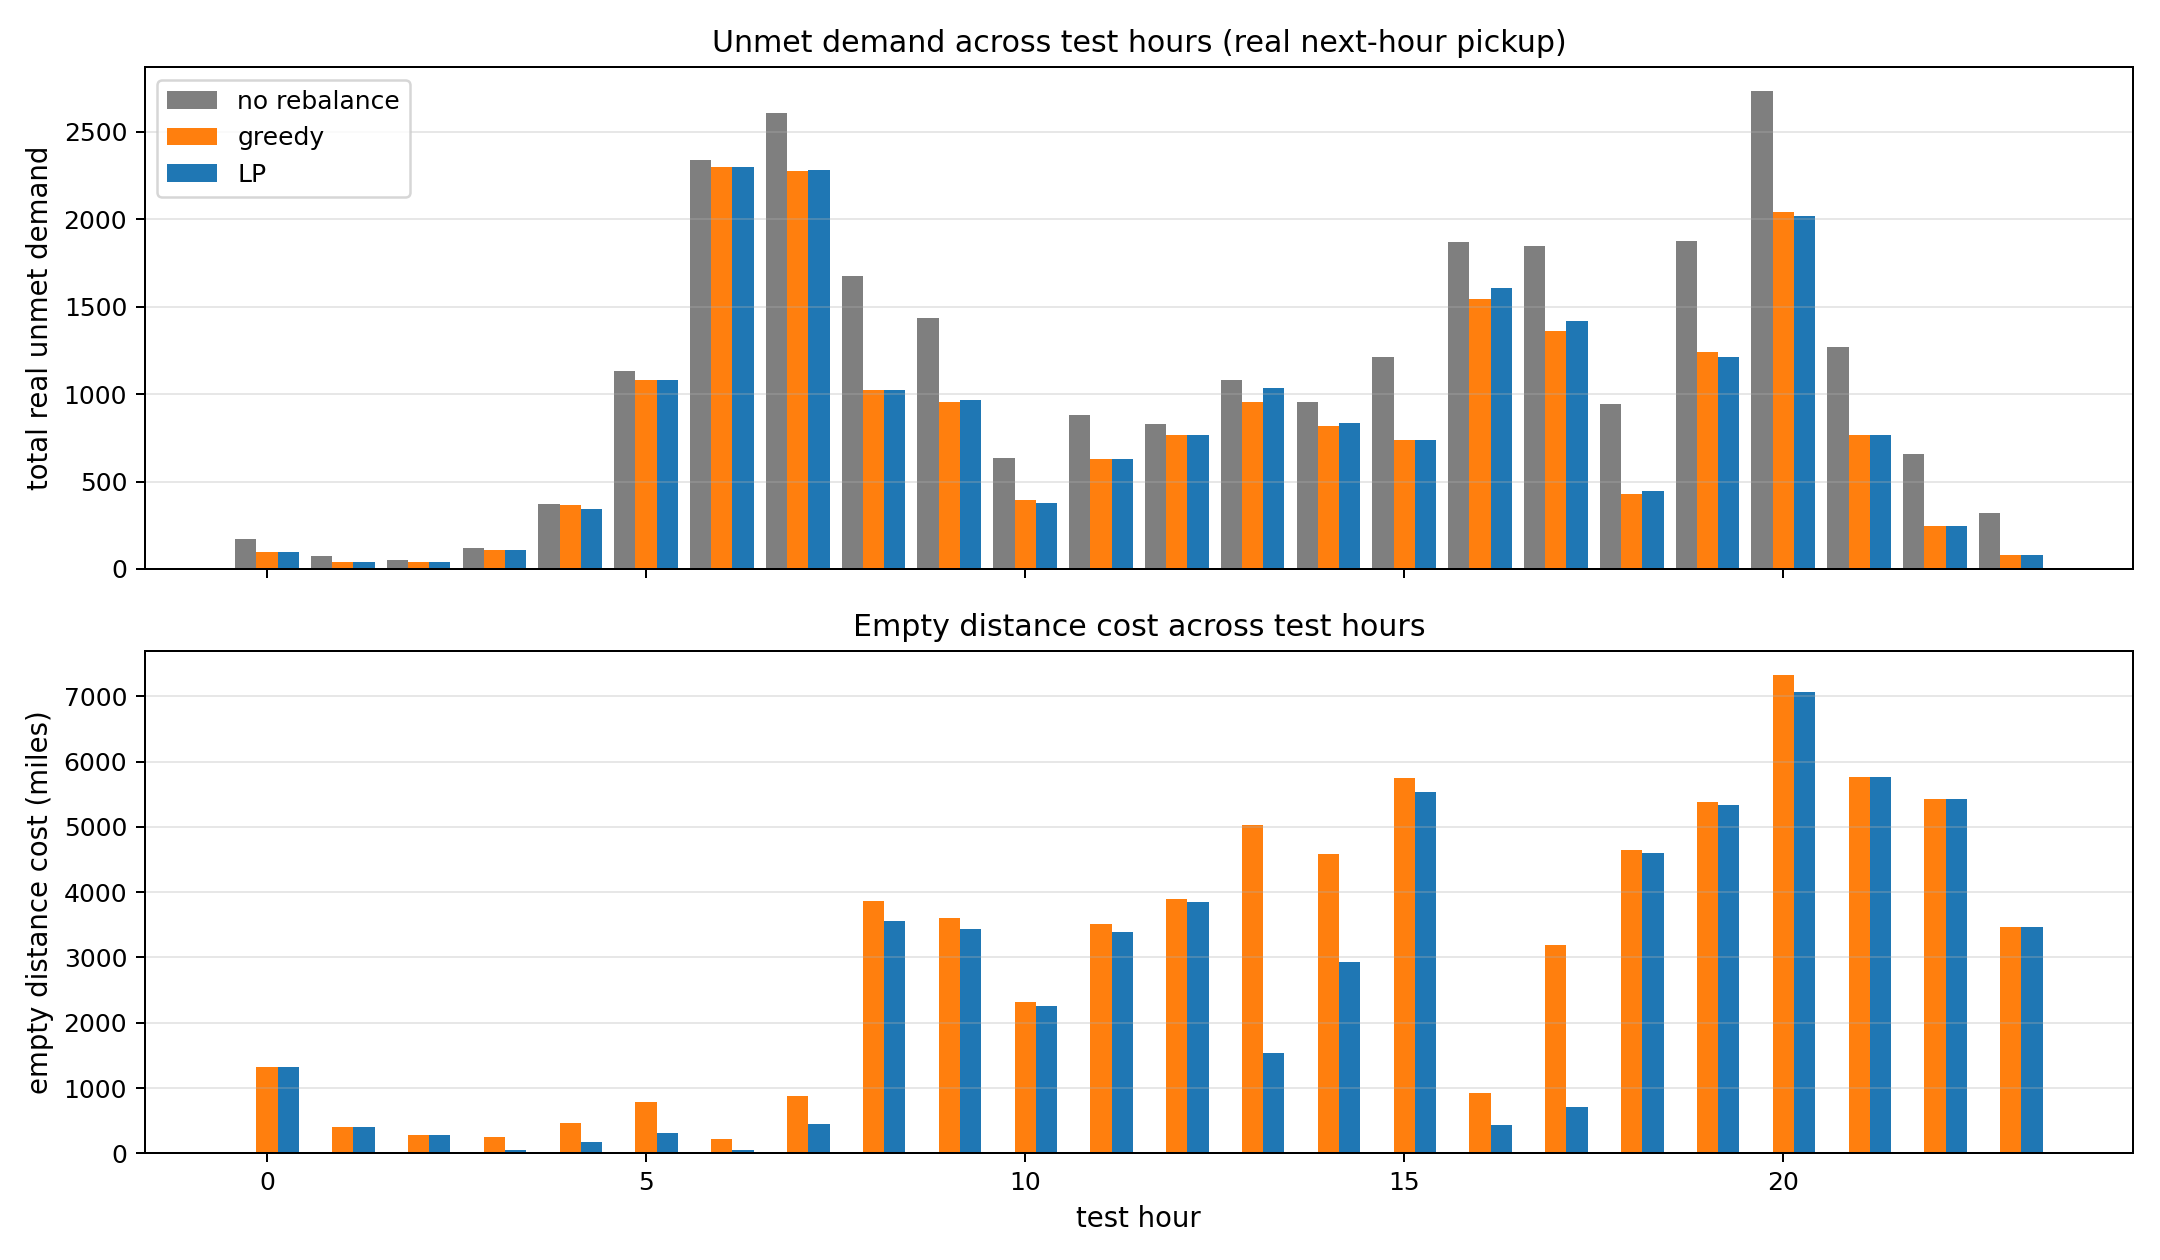
\includegraphics[width=0.85\textwidth]{../results/figures/fig_dispatch_comparison.png}
\caption{未满足需求与空驶成本在三种策略下的对比。}
\end{figure}
\end{frame}

% 10
\begin{frame}{实验结果（之二）}
\begin{figure}
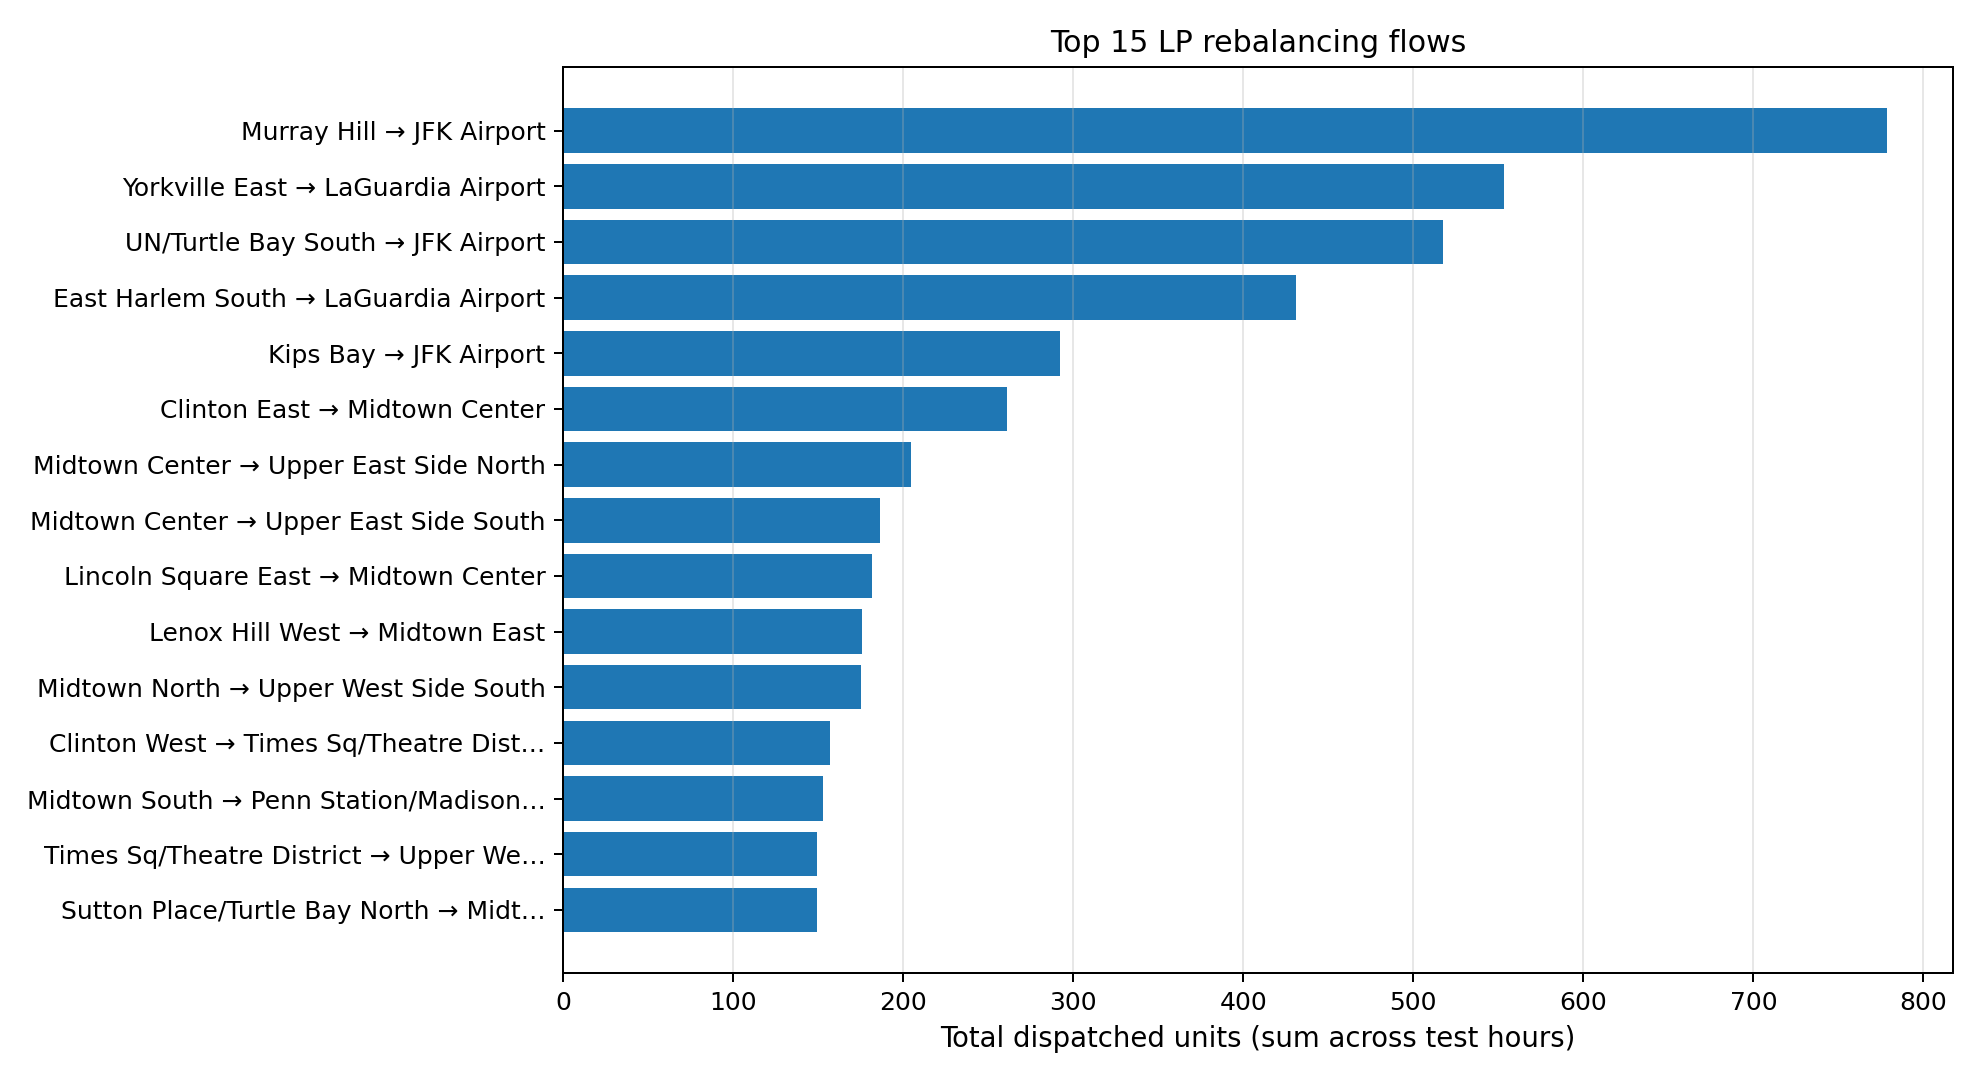
\includegraphics[width=0.85\textwidth]{../results/figures/fig_top_flows.png}
\caption{Top-10 LP 调度流量（累计于全部测试小时）。}
\end{figure}
\end{frame}

% 11
\begin{frame}{Monte Carlo 稳健性}
\begin{figure}
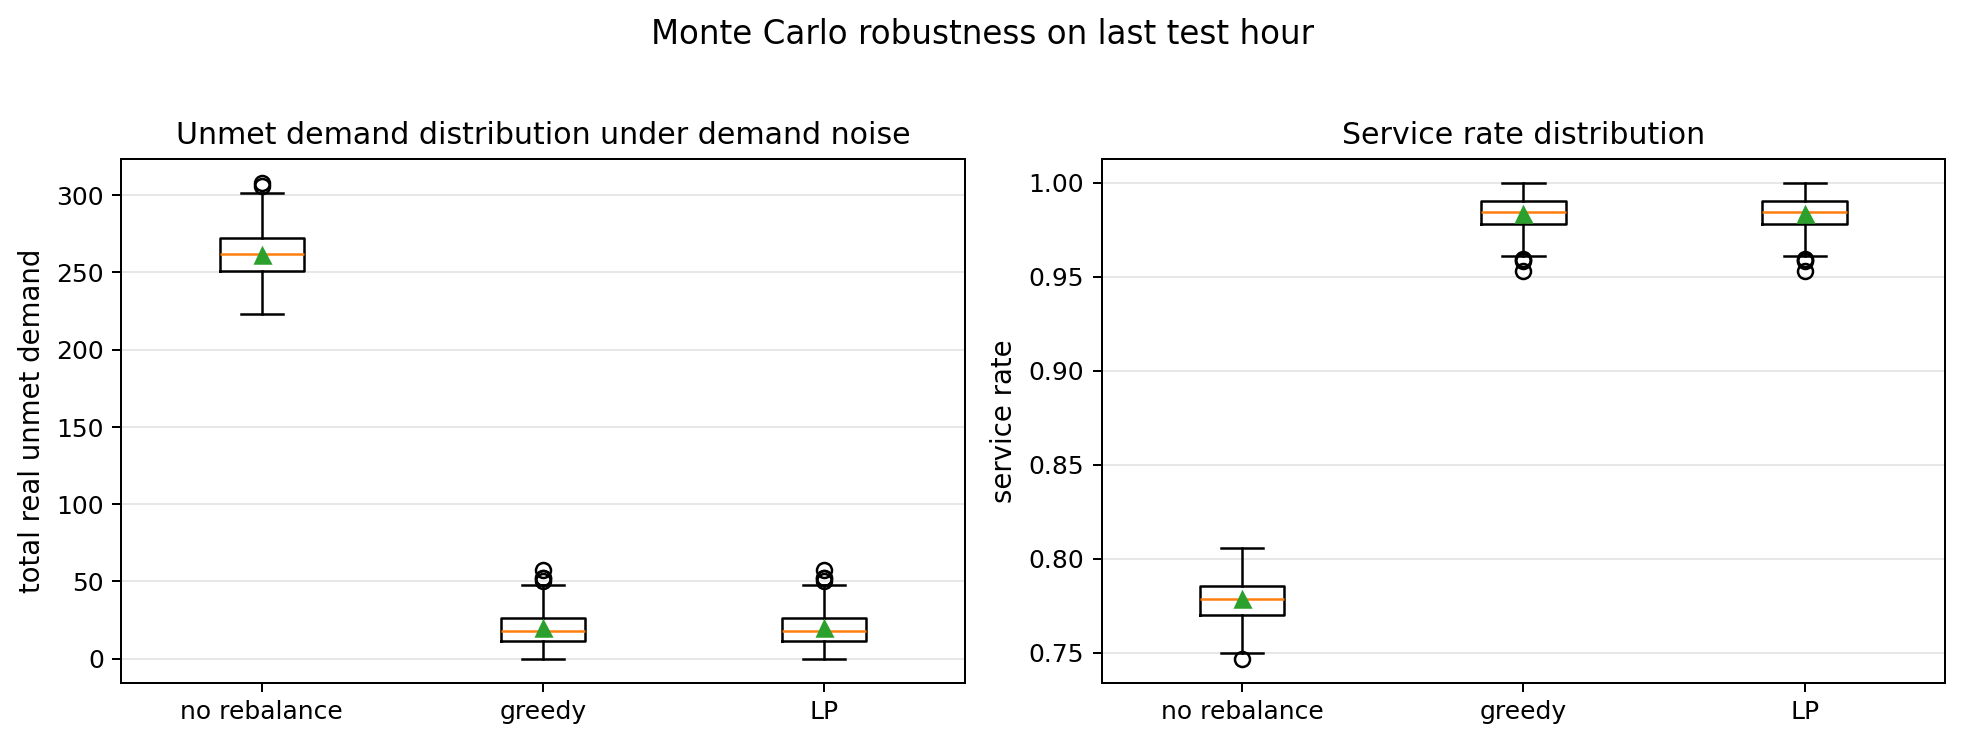
\includegraphics[width=0.85\textwidth]{../results/figures/fig_monte_carlo_boxplot.png}
\caption{固定调度方案 $X^*$ 在 200 个 Poisson 扰动场景下的指标分布。}
\end{figure}
\end{frame}

% 12
\begin{frame}{结论与局限}
\textbf{结论}：在所有测试小时上，LP $<$ greedy $<$ no-rebalance（按未满足需求）；
LP 的优势在 Monte Carlo 下保持稳定。

\vspace{0.4em}
\textbf{诚实的局限}：
\begin{itemize}\small
\item dropoff 流是供给代理 — 非真实空车库存。
\item 没有天气、道路、活动等外生数据。
\item LP 是连续 relaxation。
\item 成本矩阵未考虑实时路况。
\item 假设调度瞬时执行。
\end{itemize}

\vspace{0.4em}
完整代码：\verb|github.com/Wangxibin123/numerical_methods_2026|
\end{frame}

\begin{frame}
\begin{center}
{\Huge 谢谢}\\
\vspace{1em}
{\large 问题与讨论}
\end{center}
\end{frame}

\end{document}
